\chapter{Measurement Results}

In this chapter we discuss different combinations of MAC protocols employed on the two links. Firstly, we briefly discuss how we configured the flowgraphs to model the MAC protocols. Thereafter, we assess the measurement results where both senders employ the same MAC protocols. Eventually, we do the same where the senders employ different MAC protocols. 

\section{Flowgraph Protocol Configuration}

\paragraph{Pure ALOHA}
For pure ALOHA senders we use the flowgraph as described in Section \ref{sec:aloha-sender} and shown in Figure \ref{fig:grc-aloha-sender}. 

\paragraph{CSMA/CA}
As mentioned in Section \ref{sec:csma-transmiter} we are not featuring the optional IEEE 802.11 RTS/CTS exchange, realize DIFS and SIFS with \code{general\_timers} and the backoff with the \code{backoff} blocks.

\paragraph{1-persistent CSMA}
For 1-persistent CSMA we use the same flowgraph as for CSMA/CA and set SIFS and backoff slot times to zero. In contrast to theoretical p-persistent CSMA we sense the channel for DIFS instead of a minimal number of samples. More accurately, we could describe the protocol as "1-persistent CSMA-like with fixed sensing duration", but for brevity's sake we will refer to it as 1-persistent CSMA.  
 
\paragraph{Traffic Saturation}
If not specified otherwise all transmitters are backlogged, i.e. we have saturated traffic. In that case the time between the generation of each packet is constant and well below the RTT. When we use the term \emph{unsaturated} the time between packets generated by the \code{dummy\_source} is exponentially distributed with $\frac{1}{\lambda}=200ms$. These packets are then buffered in a \code{frame\_buffer}. For single link scenarios this leads to Poisson-distributed traffic. 

\section{Same Protocol Combinations}

Throughout this section both transmitters are executing identical flowgraphs. Generally, when both links use the same MAC protocol we expect to see comparable results for any over a sufficiently longer period of time, although small variations are also expected due to statistical and hardware-related effects and inaccuracies. 

\subsection{Pure ALOHA}

For two links with saturated ALOHA traffic we should have zero throughput, since each and every package collides. Figure \ref{fig:results-aloha-dbl} \subref{fig:results-aloha-dbl-throughput} confirms this assumption. The corresponding packet loss of 100\% is depicted in Subfigure \subref{fig:results-aloha-dbl-packet-loss}. A reference that can be read off Subfigure \subref{fig:results-aloha-dbl-throughput} value is the throughput of a single saturated ALOHA link, which is about 130 kbps. This means that the combined throughput of multiple nodes in this channel with the same underlying PHY layer can never exceed 130 kbps and we can assess how well different protocols coexist and how much efficiently they make use of the channel by comparing their joint throughput to this value. Furthermore, a physical view on the channel from the sniffer's perspective is provided in Subfigure \subref{fig:results-aloha-dbl-channel-energy}. Due to the fact that the two transmissions of the senders are not completely overlapping we can see that we don't have a single sender with observed transmission energy level around 0.0011 PU, but instead two senders, where the observed energy level of the first transmitter is around 0.0006 PU, which the channel energy CDF in Subfigure \subref{fig:results-aloha-dbl-channel-energy-cdf} confirms. Note that the share of this particular energy (0.0006 PU) in the CDF is so high, because the transmission overlap does not stay constant throughout the whole measurement, but slightly varies with each repetition.
\begin{figure}[tb]
	\label{fig:results-aloha-dbl}
	\begin{center}
		\centerline{
			\subfloat[throughput]{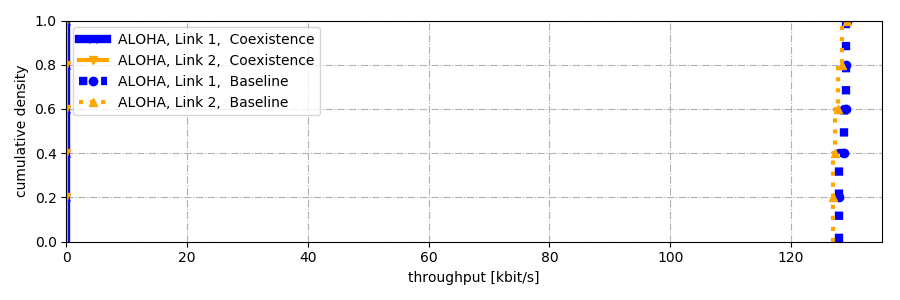
\includegraphics[width=0.52\textwidth]{pictures/results/same_combinations/aloha/throughput_cdf}\label{fig:results-aloha-dbl-throughput}}
			\subfloat[packet loss CDF]{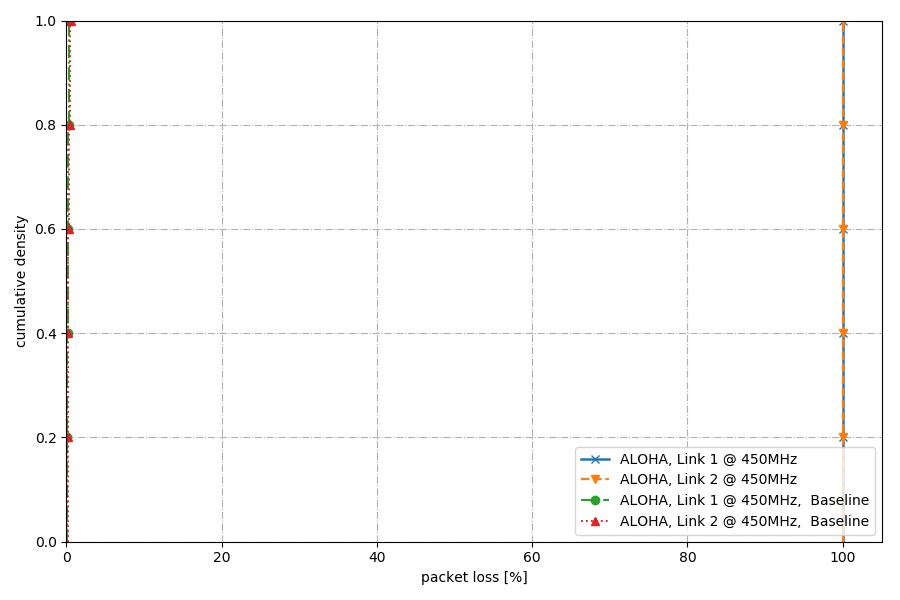
\includegraphics[width=0.52\textwidth]{pictures/results/same_combinations/aloha/packet_loss_cdf}\label{fig:results-aloha-dbl-packet-loss}}
		}		
		\centerline{
			\subfloat[channel energy]{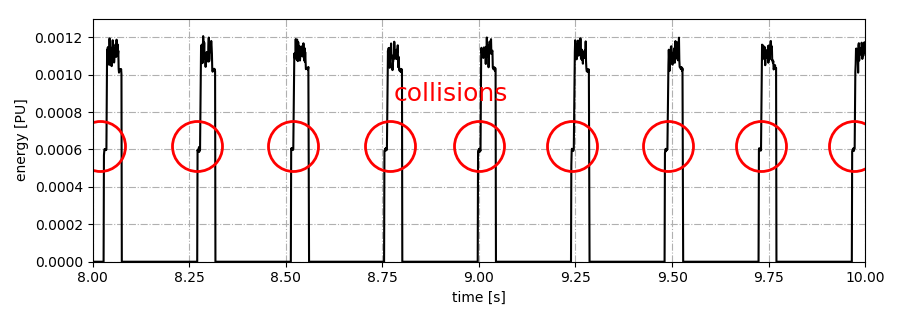
\includegraphics[width=0.52\textwidth]{pictures/results/same_combinations/aloha/smoothed_channel_energy_level_4_line_chart}\label{fig:results-aloha-dbl-channel-energy}}
			\subfloat[channel energy CDF]{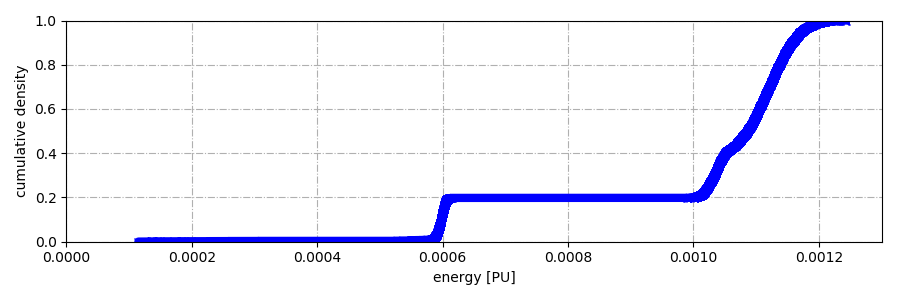
\includegraphics[width=0.52\textwidth]{pictures/results/same_combinations/aloha/smoothed_channel_energy_cdf}\label{fig:results-aloha-dbl-channel-energy-cdf}}
		}		
	\end{center}
	\caption{Measurement results for two ALOHA senders in the same channel}
\end{figure}

\clearpage

\subsection{CSMA/CA With High Parameter Set}

First of all with "high parameter set" we mean we chose high values for DIFS, SIFS and backoff slot time (BO) from which expected that they lead to good coexistence of the two links. In particular, we chose DIFS=15ms, SIFS=3ms and BO=6ms. Figure \ref{fig:results-csma-high-dbl-1} \subref{fig:results-csma-high-dbl-throughput} shows that the throughput roughly halves when two links are active at the same time. Subfigure \subref{fig:results-csma-high-dbl-throughput} shows that the frame delay roughly stays the same, where the deviation of the first link comes from packet loss related to hardware problems as described in Section \sec{label: }

\begin{figure}[tb]
	\label{fig:results-csma-high-dbl-1}
	\begin{center}
		\centerline{
			\subfloat[throughput]{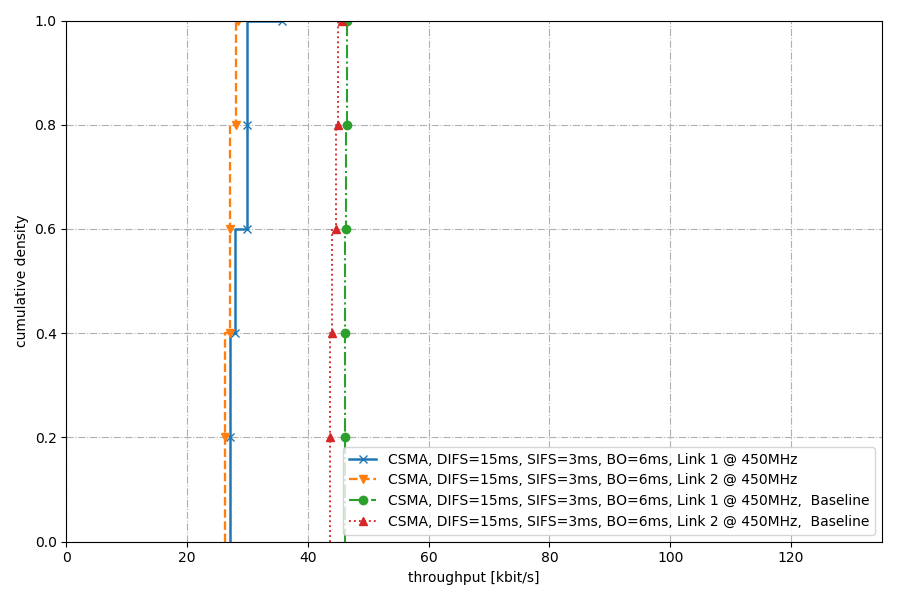
\includegraphics[width=0.6\textwidth]{pictures/results/same_combinations/csma_high_params/throughput_cdf}\label{fig:results-csma-high-dbl-throughput}}
			\subfloat[frame delay]{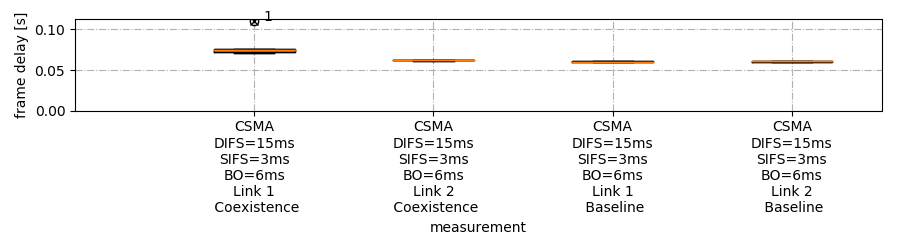
\includegraphics[width=0.6\textwidth]{pictures/results/same_combinations/csma_high_params/frame_delay_boxplot}\label{fig:results-csma-high-dbl-framedelay}}
		}	
	\end{center}
	\caption{Measurement results for the CSMA/CA with high parameter set}
\end{figure}

\begin{figure}[tb]
	\label{fig:results-csma-high-dbl-2}
	\begin{center}
		\centerline{
			\subfloat[channel energy CDF]{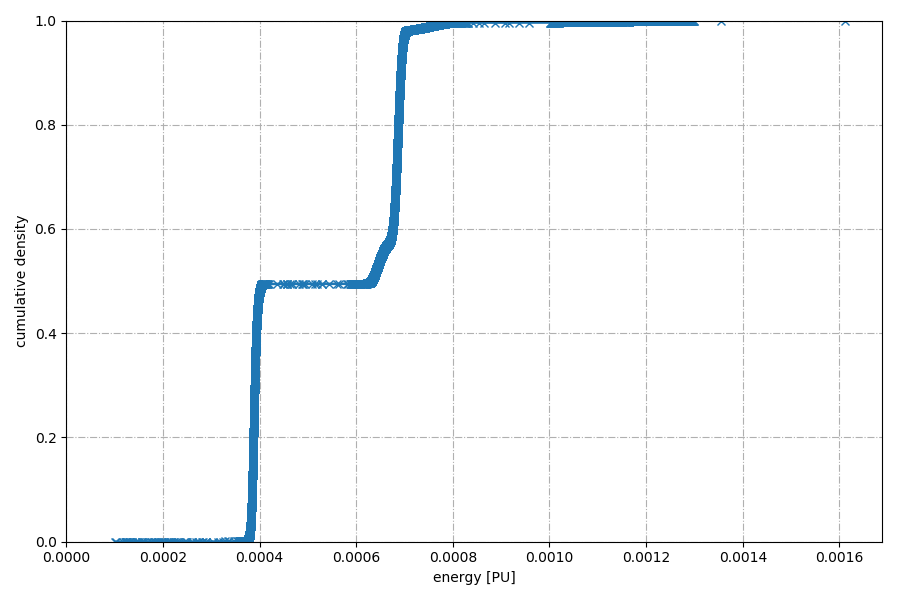
\includegraphics[width=0.6\textwidth]{pictures/results/same_combinations/csma_high_params/smoothed_channel_energy_cdf}\label{fig:results-csma-high-dbl-channel-energy}}
			\subfloat[channel energy]{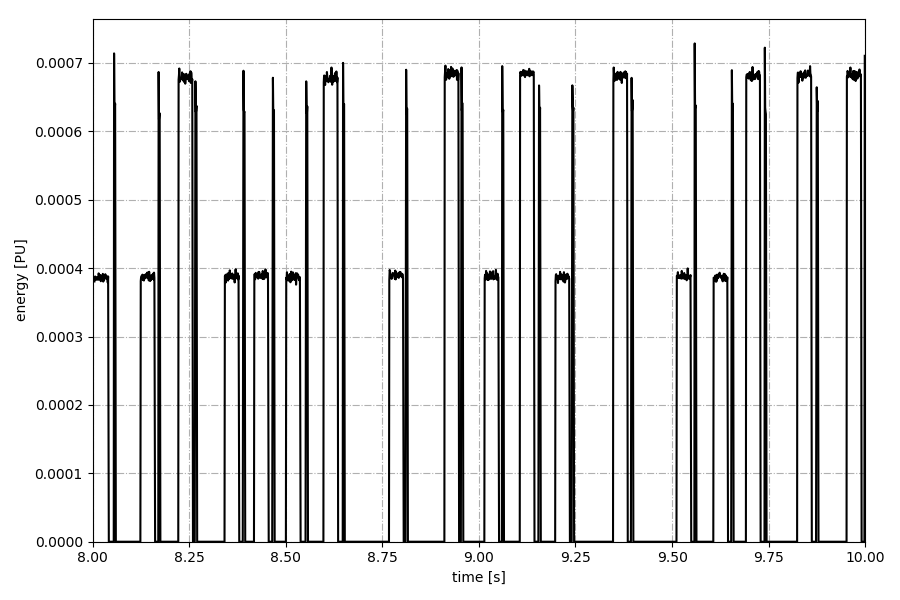
\includegraphics[width=0.6\textwidth]{pictures/results/same_combinations/csma_high_params/smoothed_channel_energy_level_4_line_chart}\label{fig:results-csma-high-dbl-channel-energy-cdf}}
		}
		\centerline{
			\subfloat[total backoff]{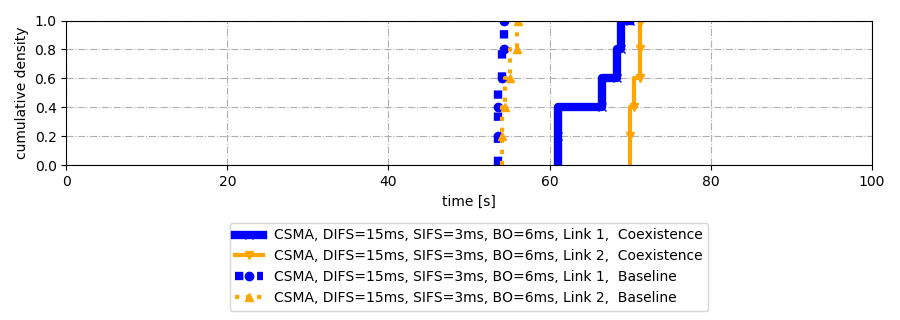
\includegraphics[width=0.6\textwidth]{pictures/results/same_combinations/csma_high_params/backoff_(joint)_sum_cdf}\label{fig:results-csma-high-dbl-backoff}}
			\subfloat[logical channel occupation]{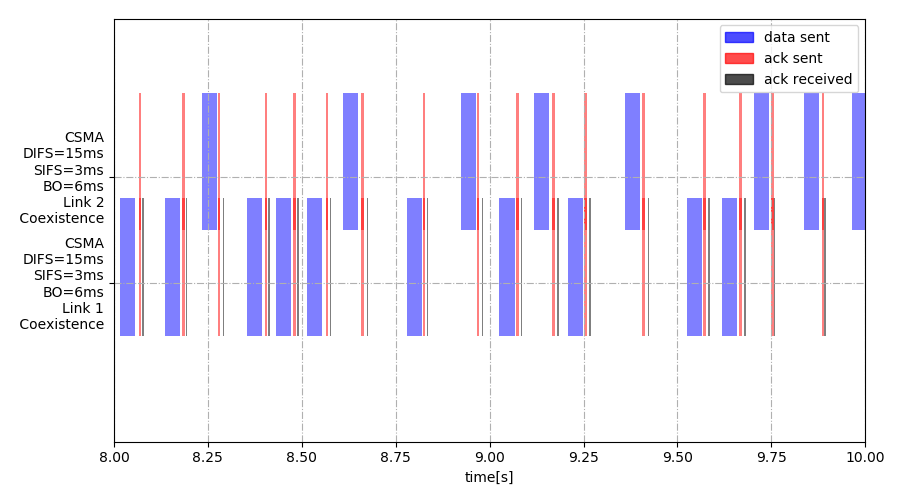
\includegraphics[width=0.6\textwidth]{pictures/results/same_combinations/csma_high_params/zoomed_channel_occupation_gantt_chart}\label{fig:results-csma-high-dbl-channel-occupation}}
		}		
	\end{center}
	\caption{Measurement results for the CSMA/CA with high parameter set}
\end{figure}

\clearpage



\subsection{CSMA/CA With Low Parameter Set}

\begin{figure}[tb]
	\label{fig:results-csma-low-dbl}
	\begin{center}
		\centerline{
			\subfloat[throughput]{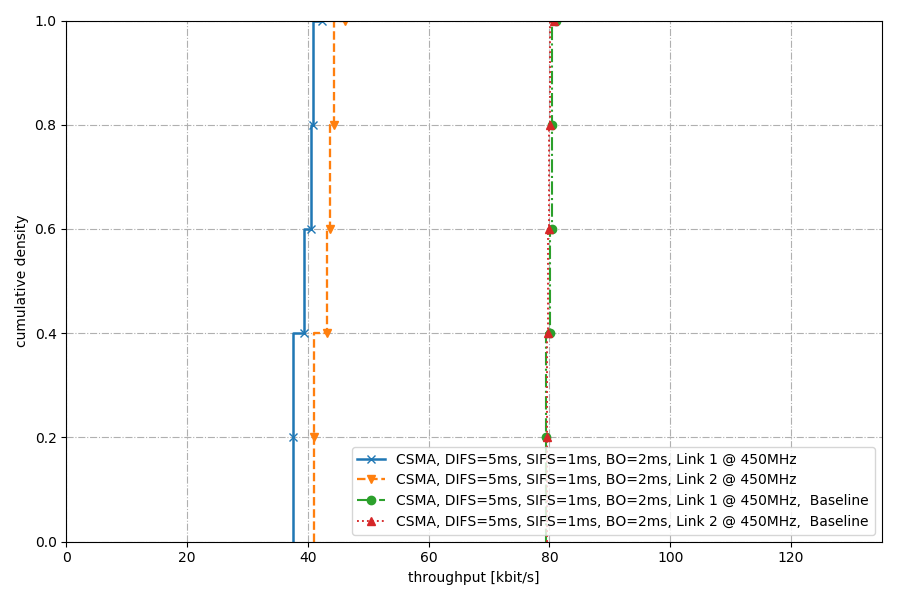
\includegraphics[width=0.6\textwidth]{pictures/results/same_combinations/csma_low_params/throughput_cdf}}
			\subfloat[frame delay]{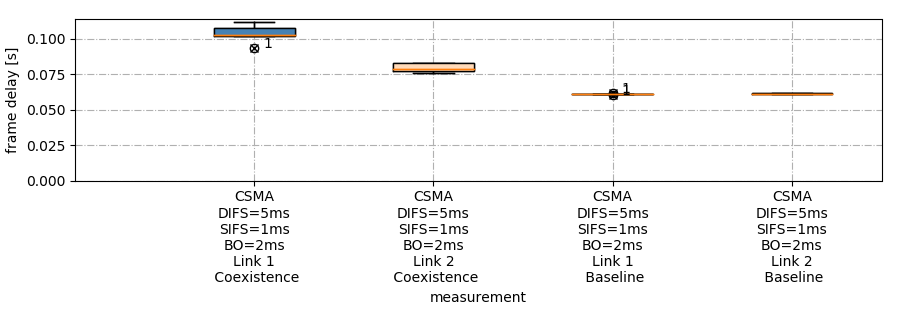
\includegraphics[width=0.6\textwidth]{pictures/results/same_combinations/csma_low_params/frame_delay_boxplot}}
		}
		\centerline{
			\subfloat[channel energy]{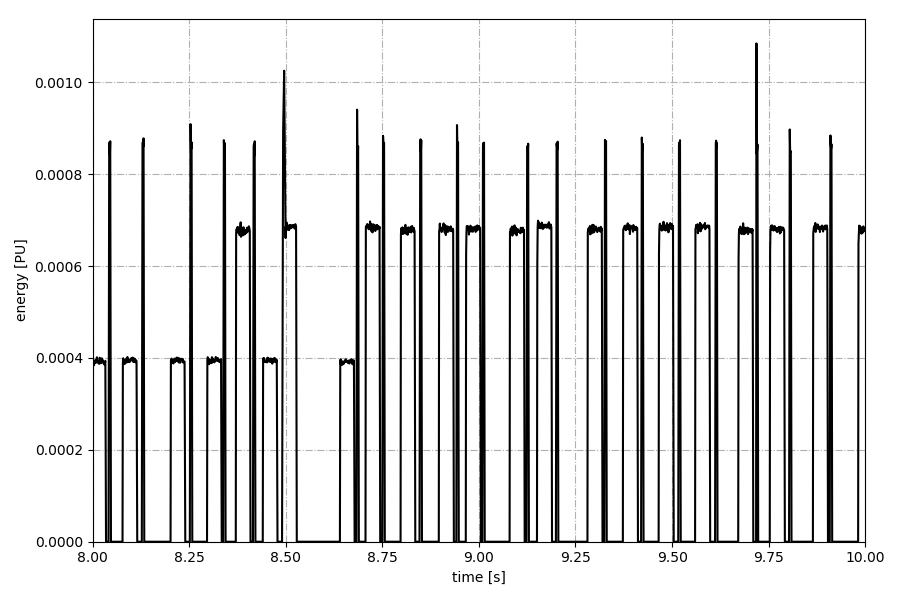
\includegraphics[width=0.6\textwidth]{pictures/results/same_combinations/csma_low_params/smoothed_channel_energy_level_4_line_chart}}
			\subfloat[channel energy CDF]{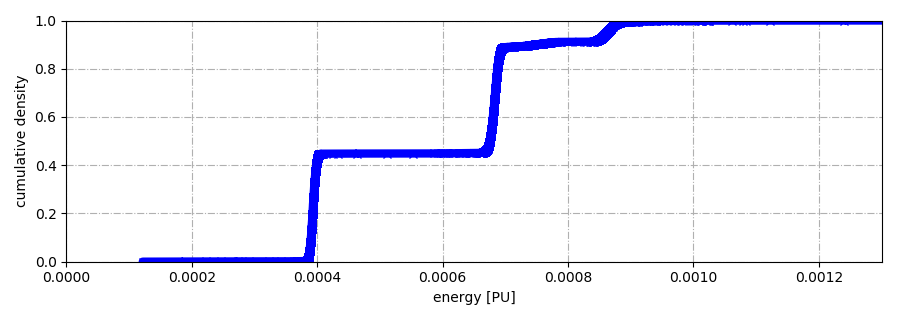
\includegraphics[width=0.6\textwidth]{pictures/results/same_combinations/csma_low_params/smoothed_channel_energy_cdf}}
		}
		\centerline{
			\subfloat[logical channel occupation]{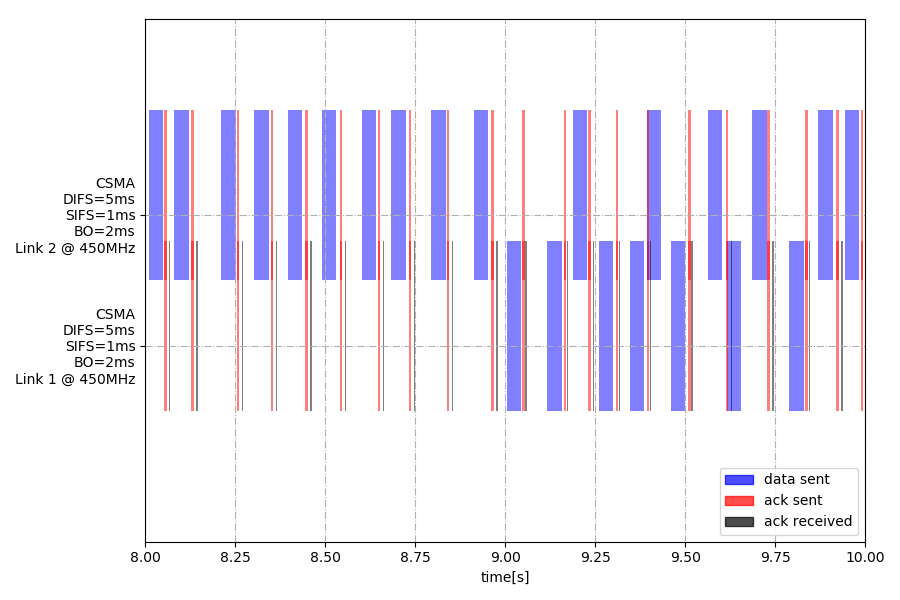
\includegraphics[width=0.6\textwidth]{pictures/results/same_combinations/csma_low_params/zoomed_channel_occupation_gantt_chart}}
			\subfloat[total backoff]{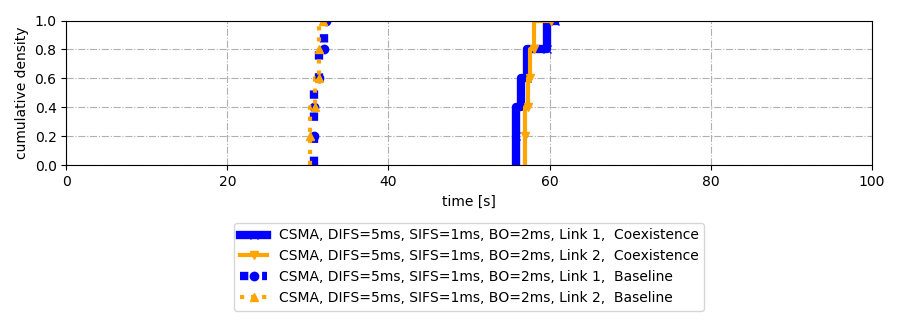
\includegraphics[width=0.6\textwidth]{pictures/results/same_combinations/csma_low_params/backoff_(joint)_sum_cdf}}
		}		
	\end{center}
	\caption{Measurement results for the CSMA/CA with low parameter set}
\end{figure}

\clearpage

\subsection{CSMA/CA With Medium Parameter Set}

\begin{figure}[tb]
	\label{fig:results-csma-med-dbl}
	\begin{center}
		\centerline{
			\subfloat[throughput]{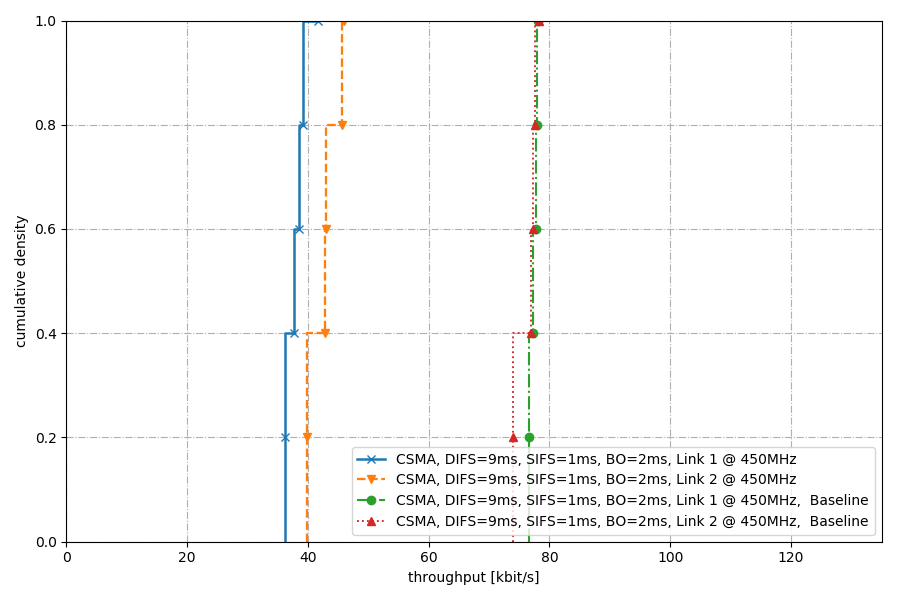
\includegraphics[width=0.6\textwidth]{pictures/results/same_combinations/csma_med_params/throughput_cdf}}
			\subfloat[frame delay]{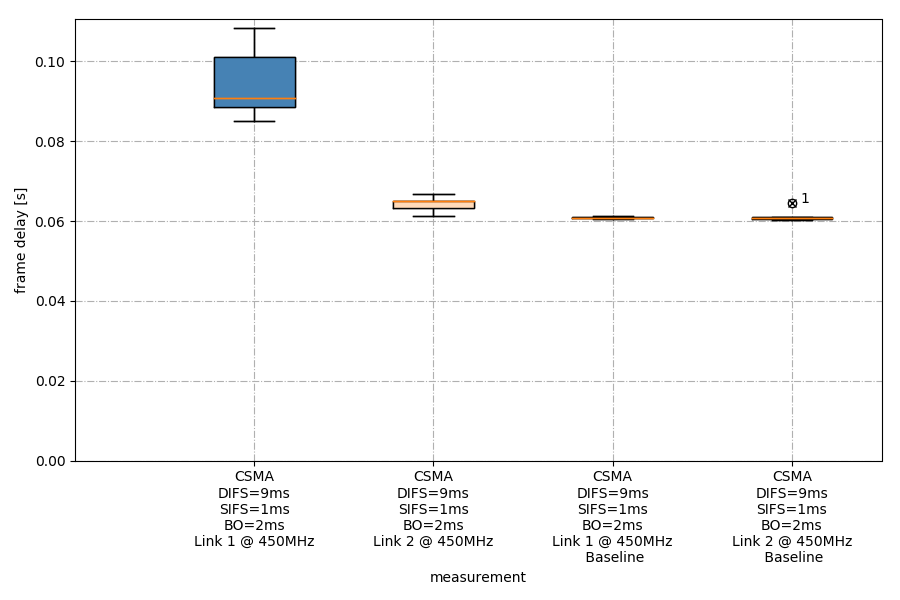
\includegraphics[width=0.6\textwidth]{pictures/results/same_combinations/csma_med_params/frame_delay_boxplot}}
		}
		\centerline{
			\subfloat[channel energy]{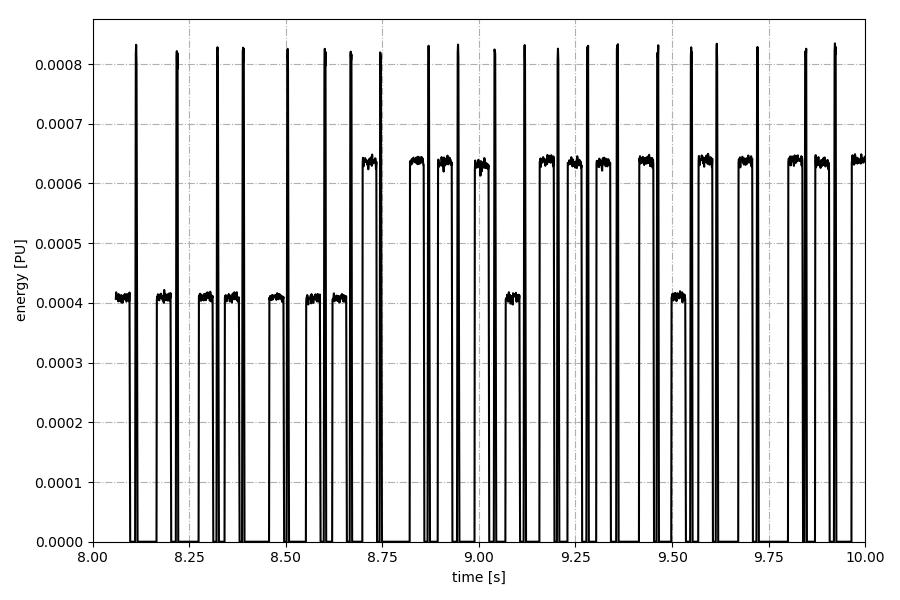
\includegraphics[width=0.6\textwidth]{pictures/results/same_combinations/csma_med_params/smoothed_channel_energy_level_4_line_chart}}
			\subfloat[channel energy CDF]{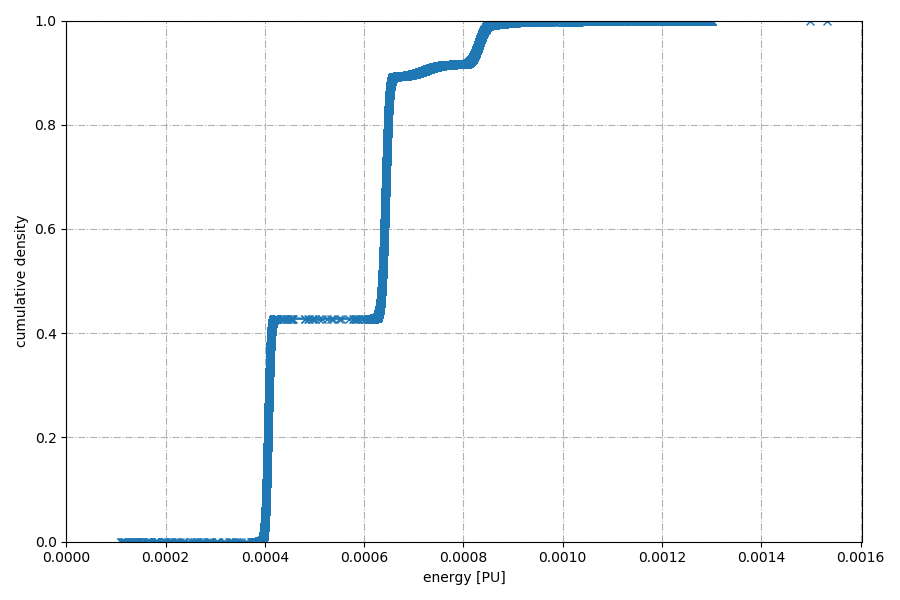
\includegraphics[width=0.6\textwidth]{pictures/results/same_combinations/csma_med_params/smoothed_channel_energy_cdf}}
		}
		\centerline{
			\subfloat[logical channel occupation]{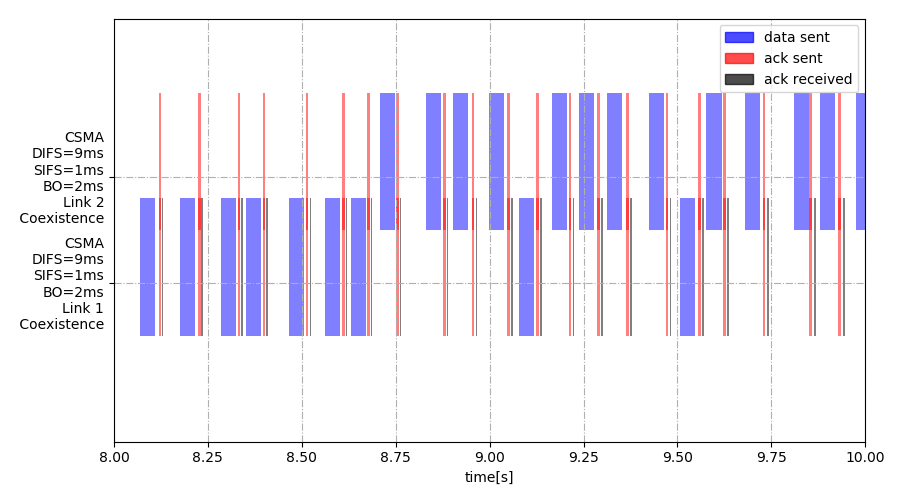
\includegraphics[width=0.6\textwidth]{pictures/results/same_combinations/csma_med_params/zoomed_channel_occupation_gantt_chart}}
			\subfloat[total backoff]{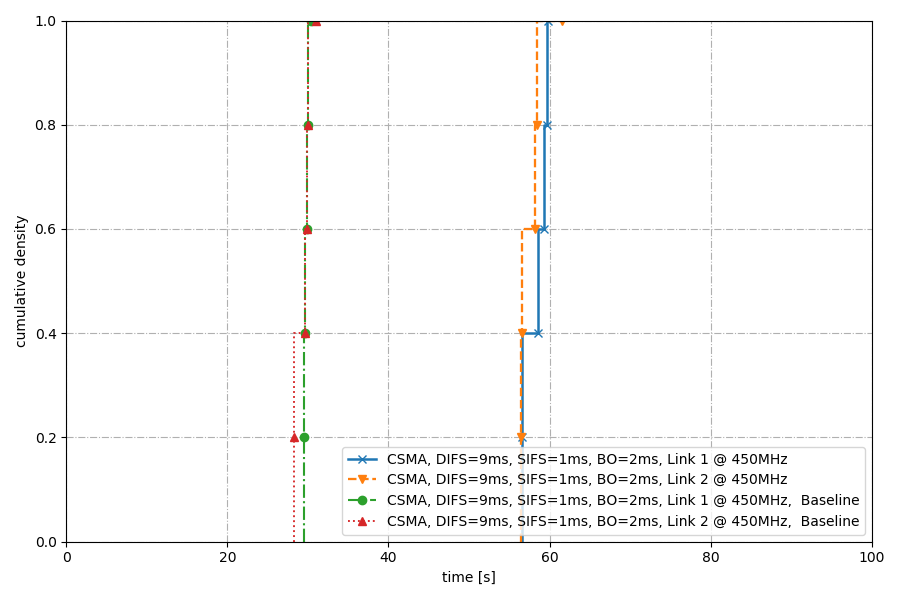
\includegraphics[width=0.6\textwidth]{pictures/results/same_combinations/csma_med_params/backoff_(joint)_sum_cdf}}
		}		
	\end{center}
	\caption{Measurement results for the CSMA/CA with medium parameter set}
\end{figure}

\clearpage



\subsection{1-persistent CSMA}

\begin{figure}[tb]
	\label{fig:results-difs-only-dbl}
	\begin{center}
		\centerline{
			\subfloat[throughput]{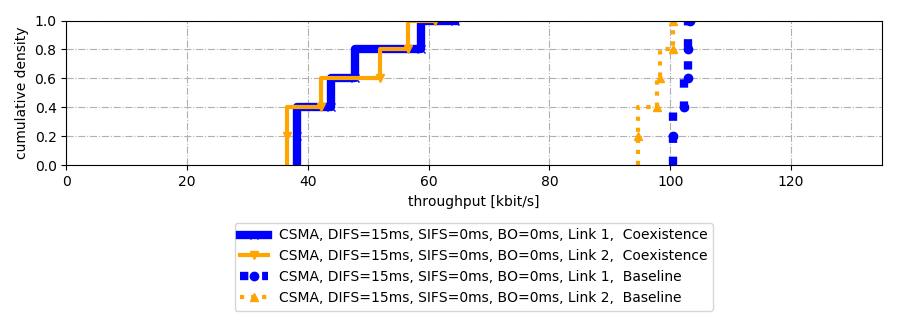
\includegraphics[width=0.6\textwidth]{pictures/results/same_combinations/difs_only/throughput_cdf}}
			\subfloat[frame delay]{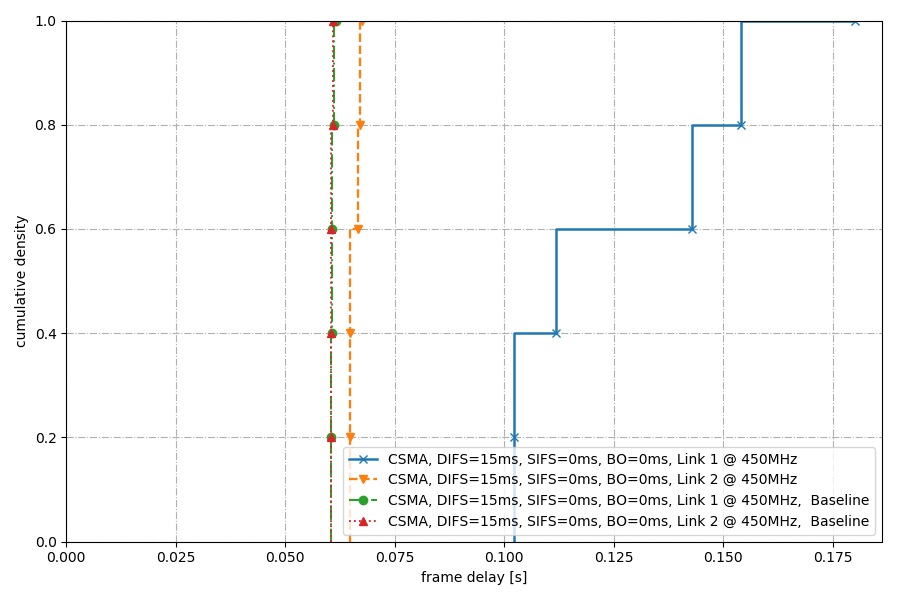
\includegraphics[width=0.6\textwidth]{pictures/results/same_combinations/difs_only/frame_delay_cdf}}
		}
		\centerline{
			\subfloat[Channel Energy]{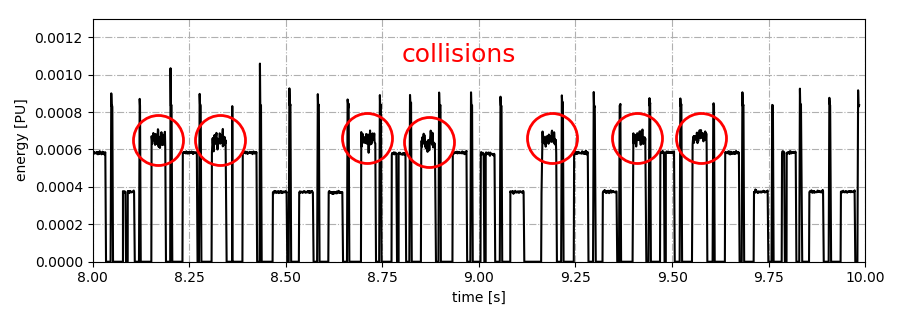
\includegraphics[width=0.6\textwidth]{pictures/results/same_combinations/difs_only/smoothed_channel_energy_level_4_line_chart}}
			\subfloat[Channel Energy CDF]{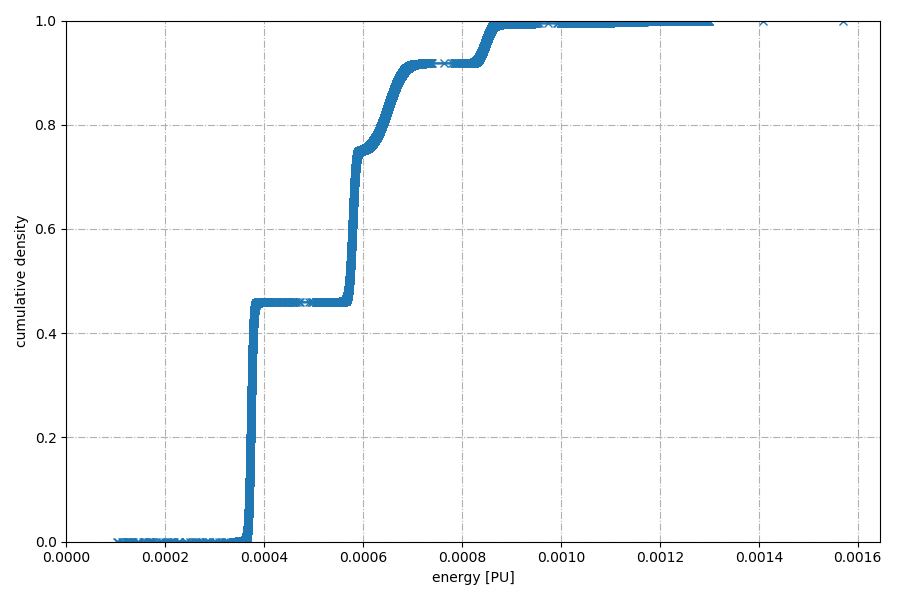
\includegraphics[width=0.6\textwidth]{pictures/results/same_combinations/difs_only/smoothed_channel_energy_cdf}}
		}
		\centerline{
			\subfloat[Logical Channel Occupation]{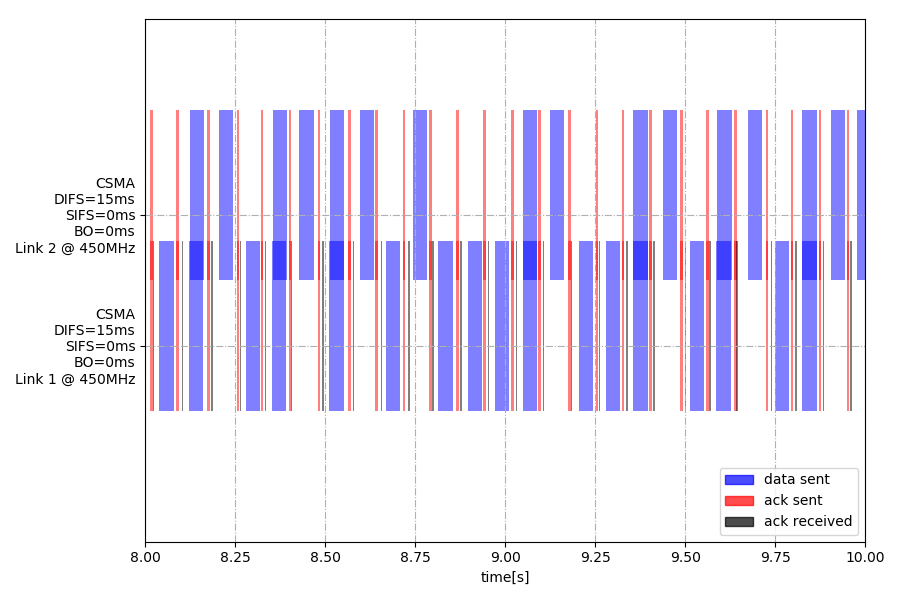
\includegraphics[width=0.6\textwidth]{pictures/results/same_combinations/difs_only/zoomed_channel_occupation_gantt_chart}}
			\subfloat[Total Backoff]{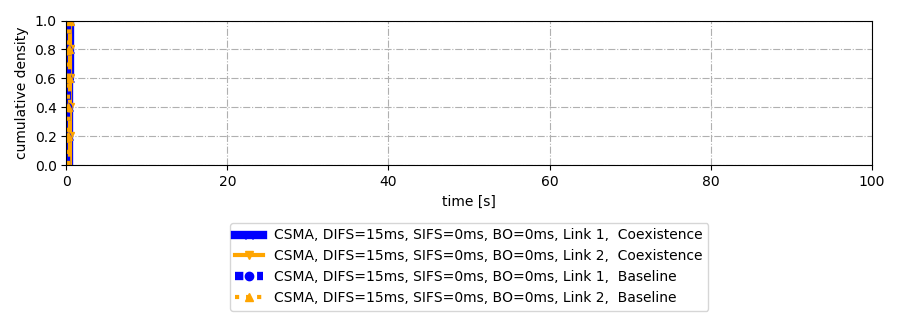
\includegraphics[width=0.6\textwidth]{pictures/results/same_combinations/difs_only/backoff_(joint)_sum_cdf}}
		}		
	\end{center}
	\caption{Measurement results for 1-persistent CSMA/CA}
\end{figure}

\clearpage




\section{Different Protocol Combinations}

%flawed
\subsection{ALOHA and CSMA/CA}

\begin{figure}[tb]
	\label{fig:results-aloha-csma}
	\begin{center}
		\centerline{
			\subfloat[Throughput]{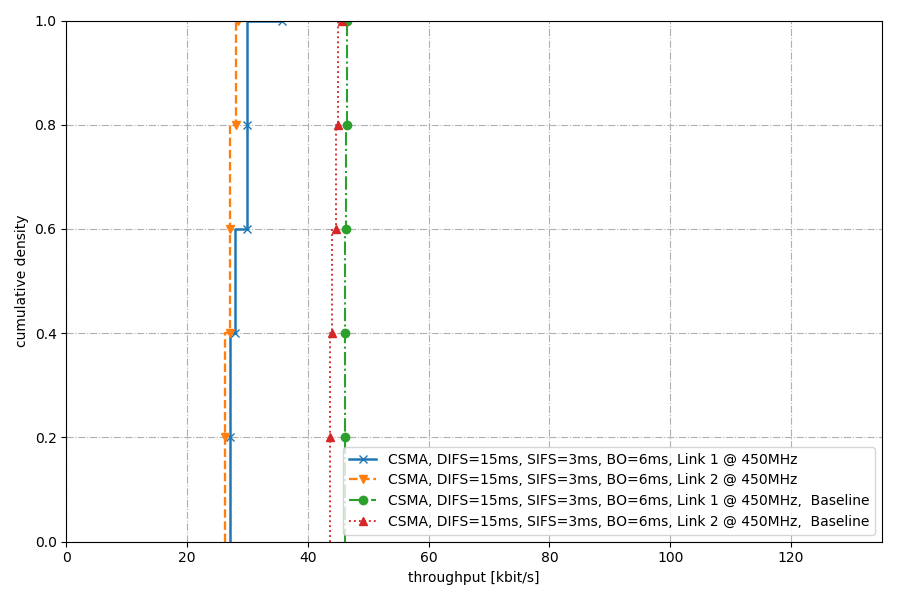
\includegraphics[width=0.6\textwidth]{pictures/results/same_combinations/csma_high_params/throughput_cdf}}
			\subfloat[RTT]{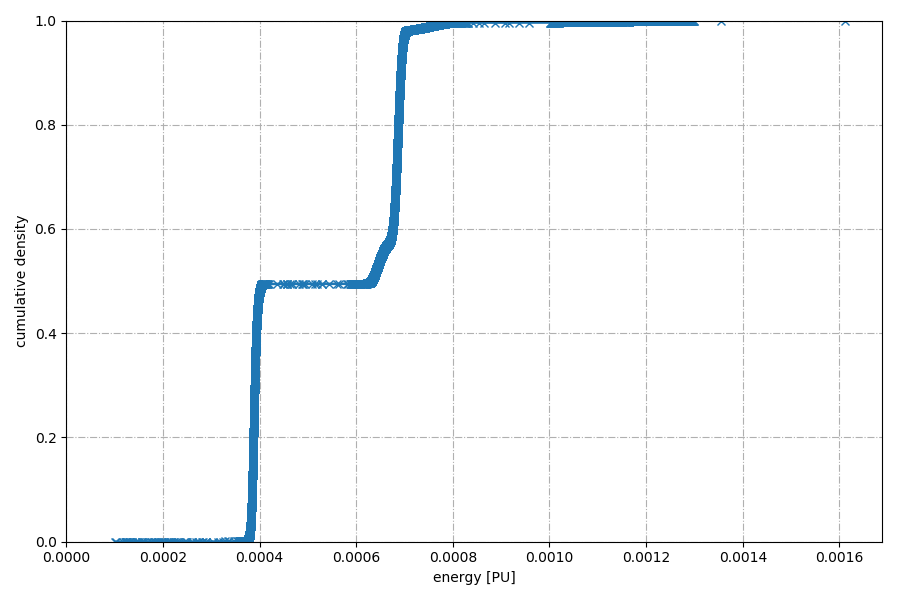
\includegraphics[width=0.6\textwidth]{pictures/results/same_combinations/csma_high_params/smoothed_channel_energy_cdf}}
		}
		\centerline{
			\subfloat[Channel Energy]{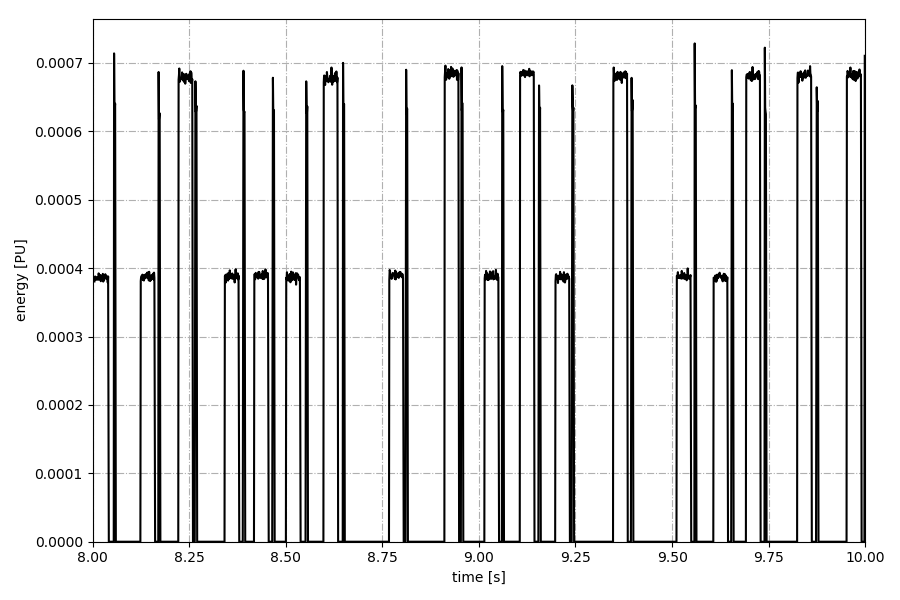
\includegraphics[width=0.6\textwidth]{pictures/results/same_combinations/csma_high_params/smoothed_channel_energy_level_4_line_chart}}
			\subfloat[Channel Energy CDF]{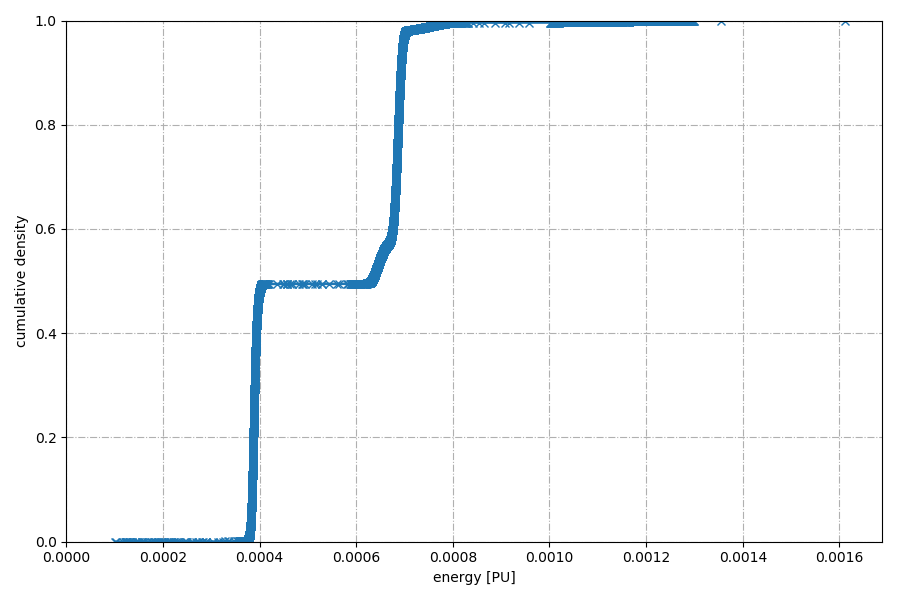
\includegraphics[width=0.6\textwidth]{pictures/results/same_combinations/csma_high_params/smoothed_channel_energy_cdf}}
		}
		\centerline{
			\subfloat[Logical Channel Occupation]{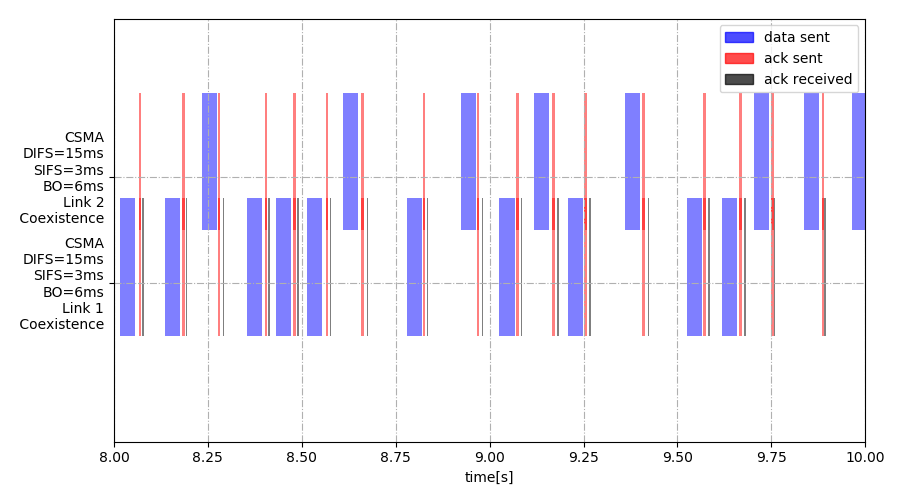
\includegraphics[width=0.6\textwidth]{pictures/results/same_combinations/csma_high_params/zoomed_channel_occupation_gantt_chart}}
			\subfloat[Total Backoff]{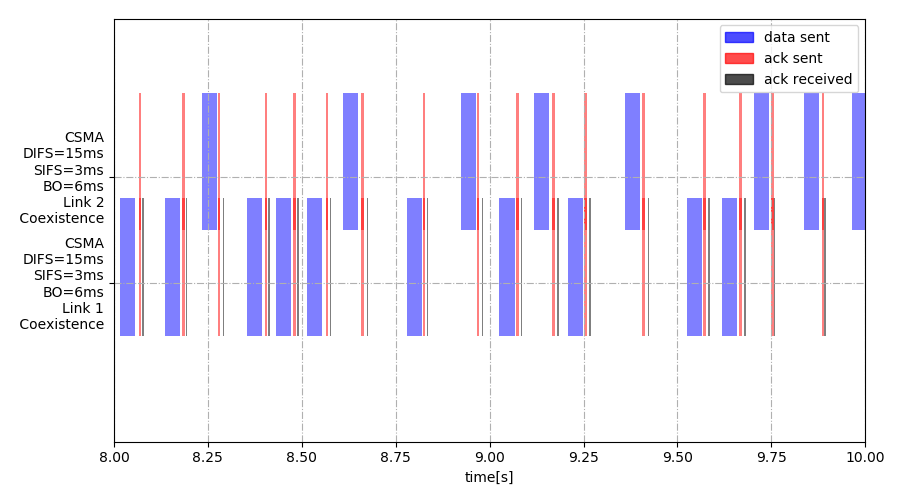
\includegraphics[width=0.6\textwidth]{pictures/results/same_combinations/csma_high_params/zoomed_channel_occupation_gantt_chart}}
		}		
	\end{center}
	\caption{Measurement results for the CSMA/CA with large parameter set}
\end{figure}

\clearpage



\subsection{Unsaturated ALOHA and CSMA/CA}

\begin{figure}[tb]
	\label{fig:results-unsat-aloha-csma}
	\begin{center}
		\centerline{
			\subfloat[Throughput]{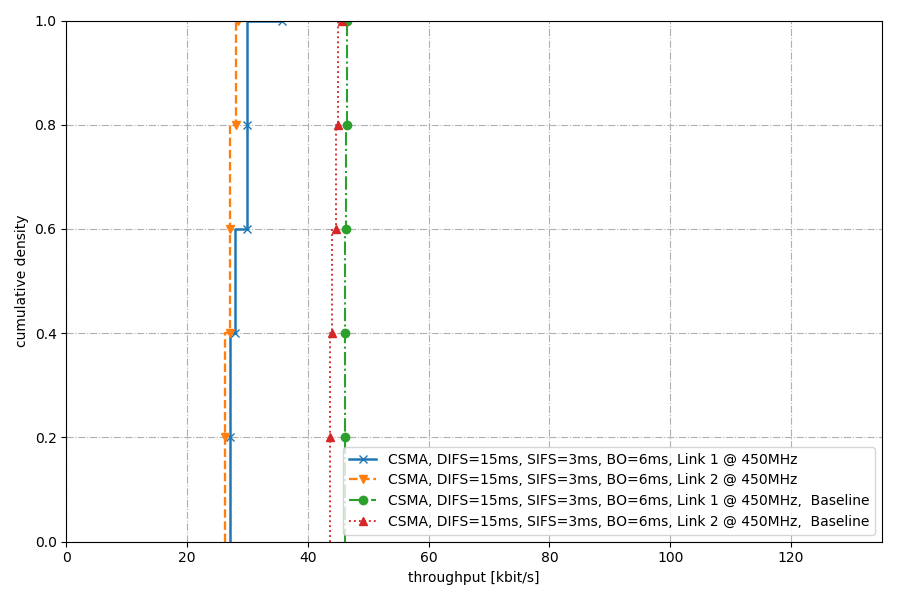
\includegraphics[width=0.6\textwidth]{pictures/results/same_combinations/csma_high_params/throughput_cdf}}
			\subfloat[RTT]{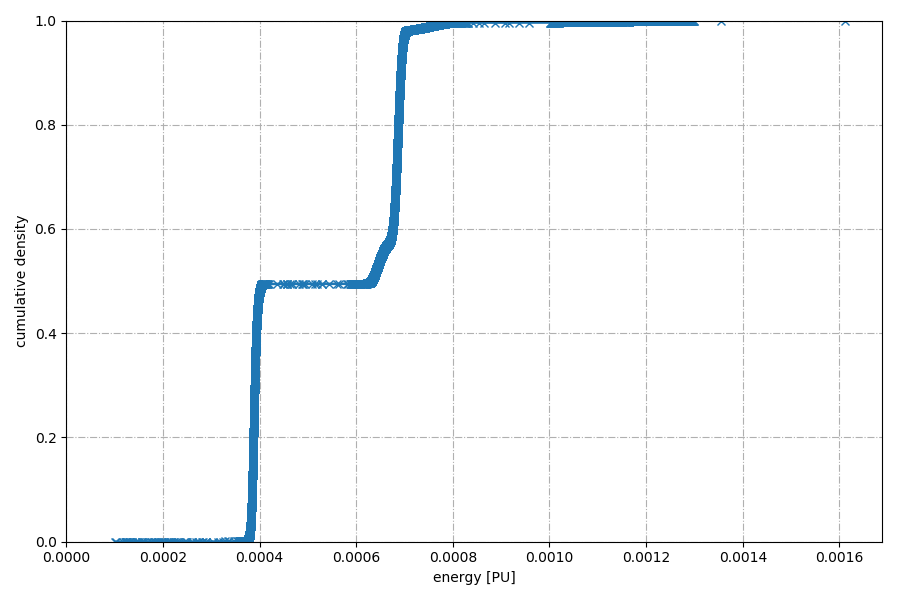
\includegraphics[width=0.6\textwidth]{pictures/results/same_combinations/csma_high_params/smoothed_channel_energy_cdf}}
		}
		\centerline{
			\subfloat[Channel Energy]{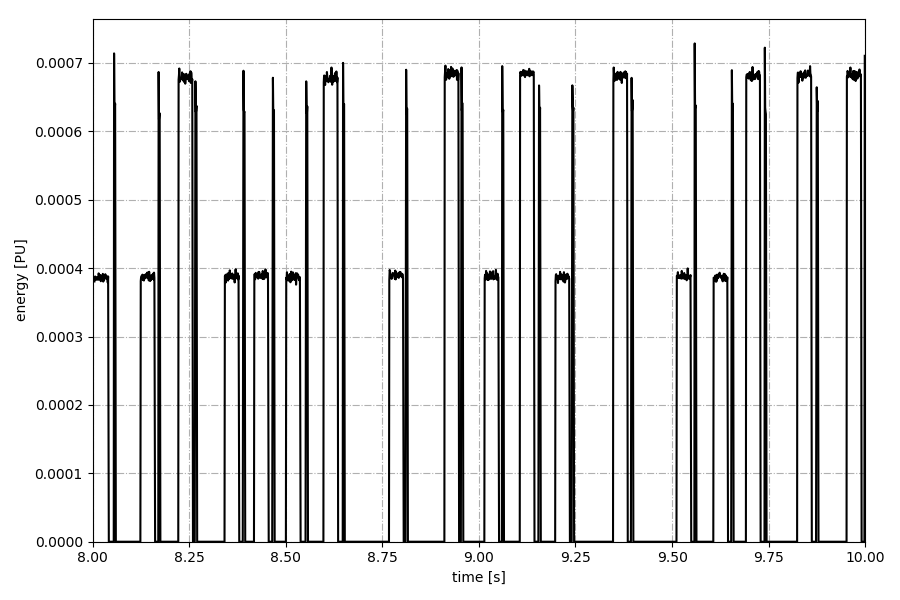
\includegraphics[width=0.6\textwidth]{pictures/results/same_combinations/csma_high_params/smoothed_channel_energy_level_4_line_chart}}
			\subfloat[Channel Energy CDF]{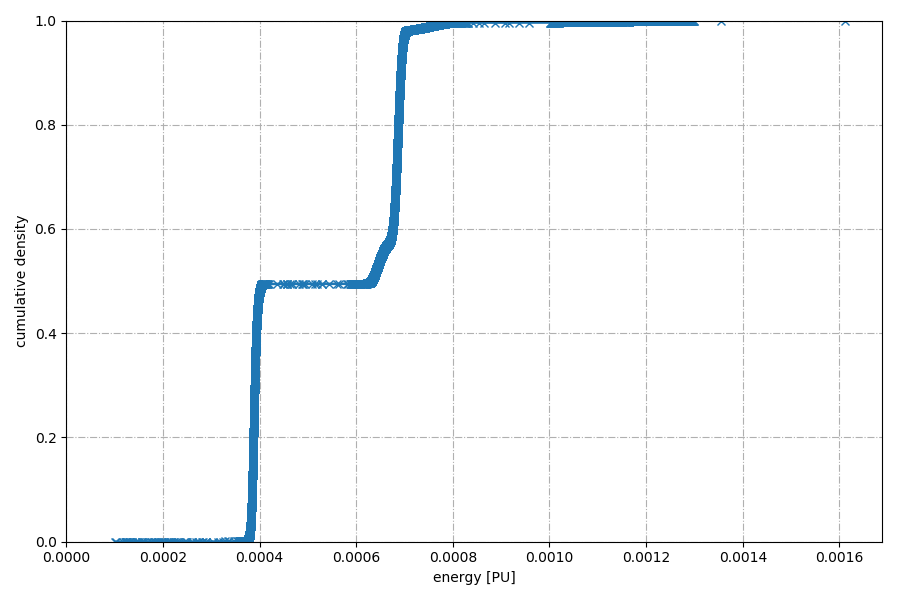
\includegraphics[width=0.6\textwidth]{pictures/results/same_combinations/csma_high_params/smoothed_channel_energy_cdf}}
		}
		\centerline{
			\subfloat[Logical Channel Occupation]{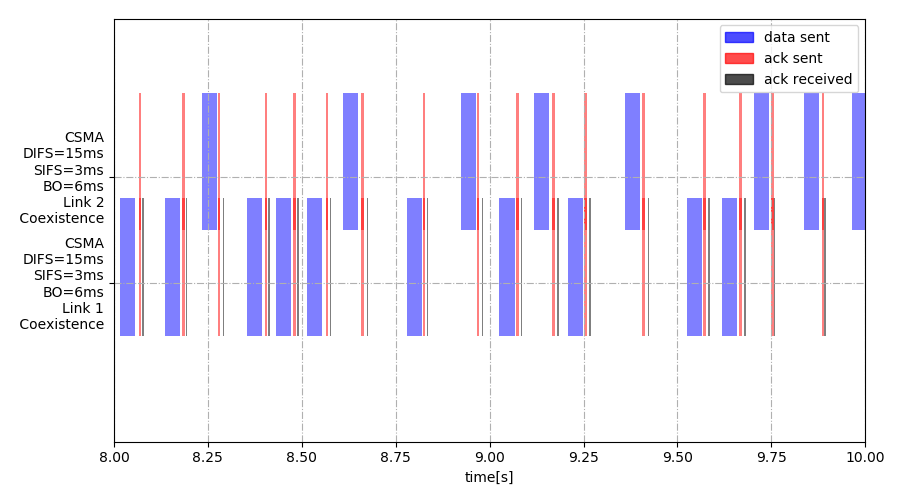
\includegraphics[width=0.6\textwidth]{pictures/results/same_combinations/csma_high_params/zoomed_channel_occupation_gantt_chart}}
			\subfloat[Total Backoff]{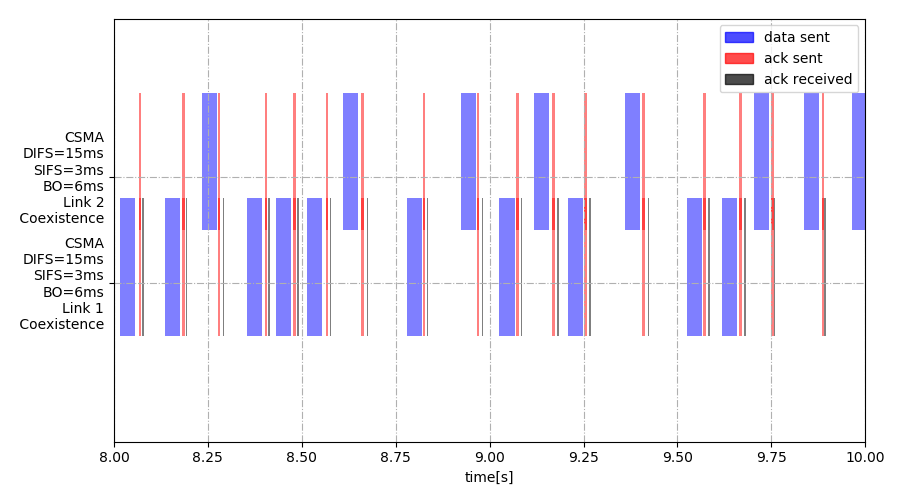
\includegraphics[width=0.6\textwidth]{pictures/results/same_combinations/csma_high_params/zoomed_channel_occupation_gantt_chart}}
		}		
	\end{center}
	\caption{Measurement results for the CSMA/CA with large parameter set}
\end{figure}

\clearpage




\subsection{Inhomogeneous CSMA/CA }



\subsection{1-persistent CSMA and ALOHA}

\begin{figure}[tb]
	\label{fig:results-difs-aloha}
	\begin{center}
		\centerline{
			\subfloat[Throughput]{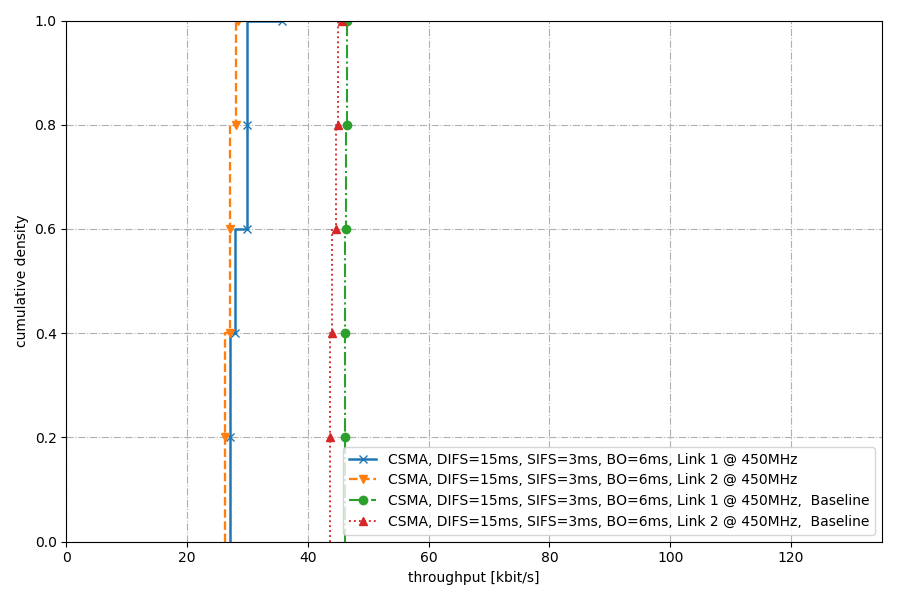
\includegraphics[width=0.6\textwidth]{pictures/results/same_combinations/csma_high_params/throughput_cdf}}
			\subfloat[RTT]{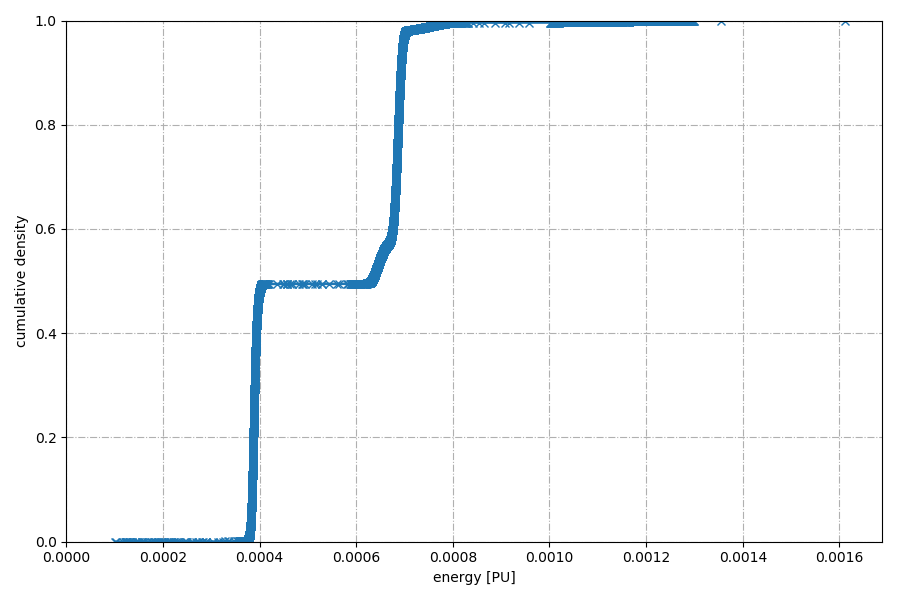
\includegraphics[width=0.6\textwidth]{pictures/results/same_combinations/csma_high_params/smoothed_channel_energy_cdf}}
		}
		\centerline{
			\subfloat[Channel Energy]{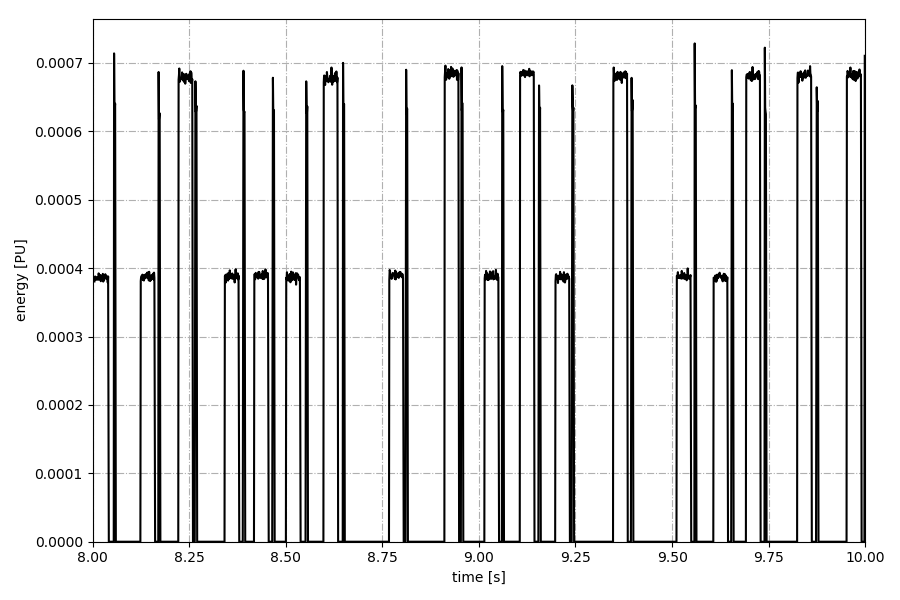
\includegraphics[width=0.6\textwidth]{pictures/results/same_combinations/csma_high_params/smoothed_channel_energy_level_4_line_chart}}
			\subfloat[Channel Energy CDF]{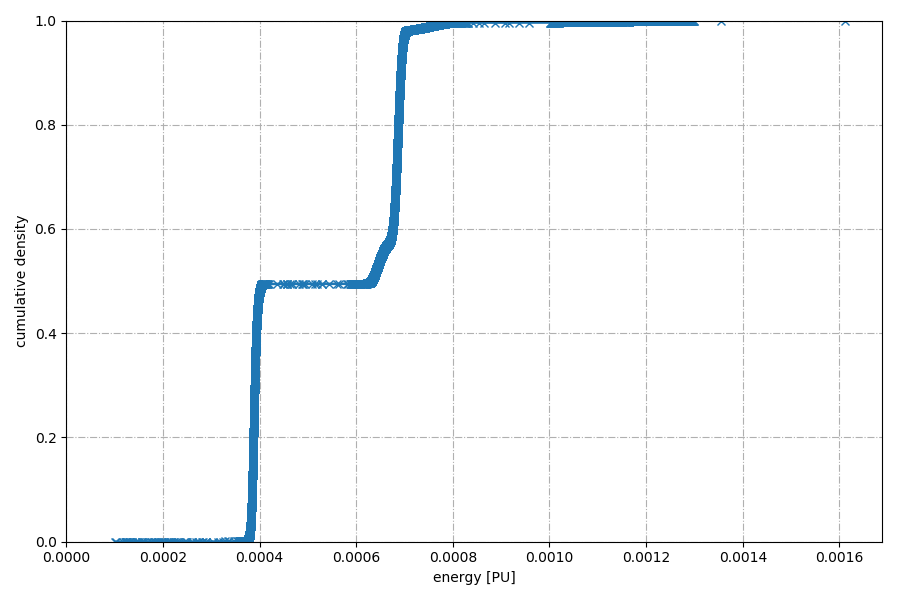
\includegraphics[width=0.6\textwidth]{pictures/results/same_combinations/csma_high_params/smoothed_channel_energy_cdf}}
		}
		\centerline{
			\subfloat[Logical Channel Occupation]{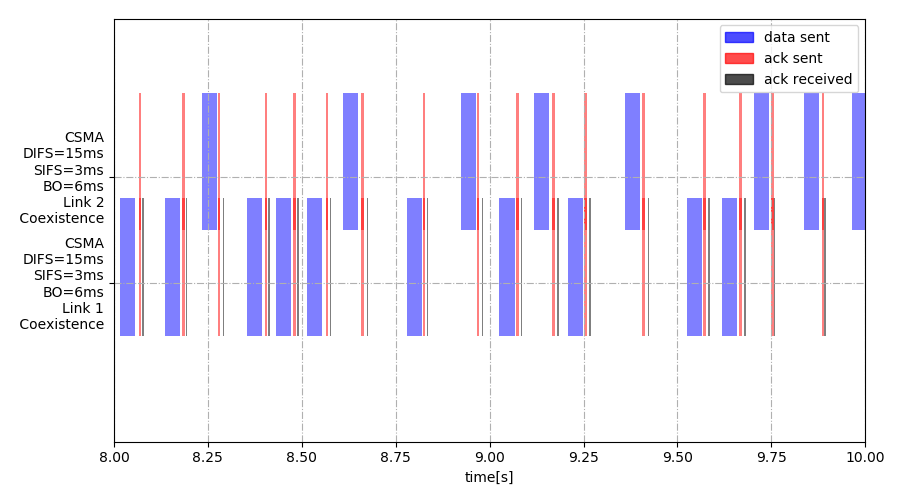
\includegraphics[width=0.6\textwidth]{pictures/results/same_combinations/csma_high_params/zoomed_channel_occupation_gantt_chart}}
			\subfloat[Total Backoff]{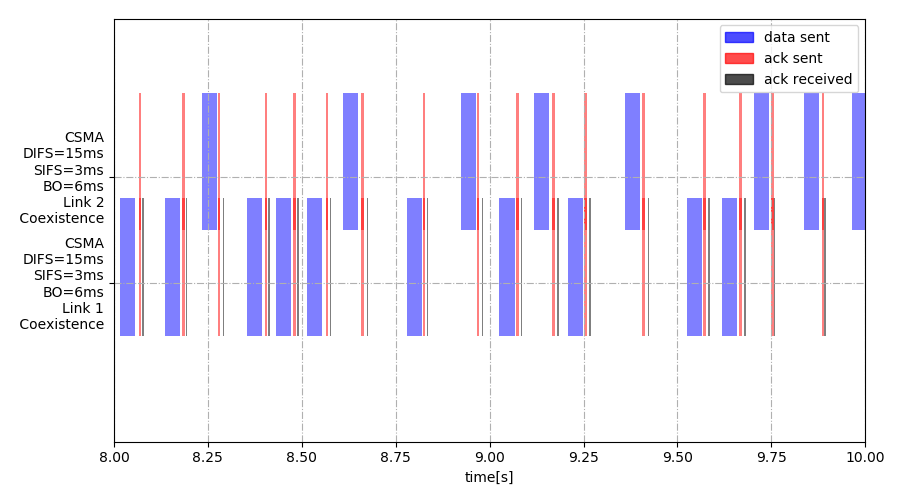
\includegraphics[width=0.6\textwidth]{pictures/results/same_combinations/csma_high_params/zoomed_channel_occupation_gantt_chart}}
		}		
	\end{center}
	\caption{Measurement results for the CSMA/CA with large parameter set}
\end{figure}

\clearpage



\subsection{1-persistent CSMA and CSMA/CA}

\begin{figure}[tb]
	\label{fig:results-difs-csma}
	\begin{center}
		\centerline{
			\subfloat[Throughput]{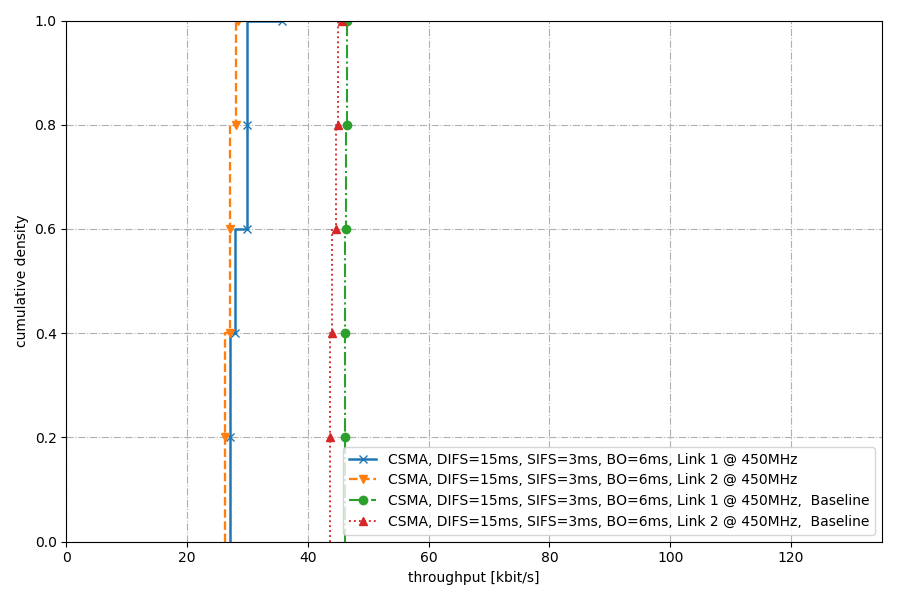
\includegraphics[width=0.6\textwidth]{pictures/results/same_combinations/csma_high_params/throughput_cdf}}
			\subfloat[RTT]{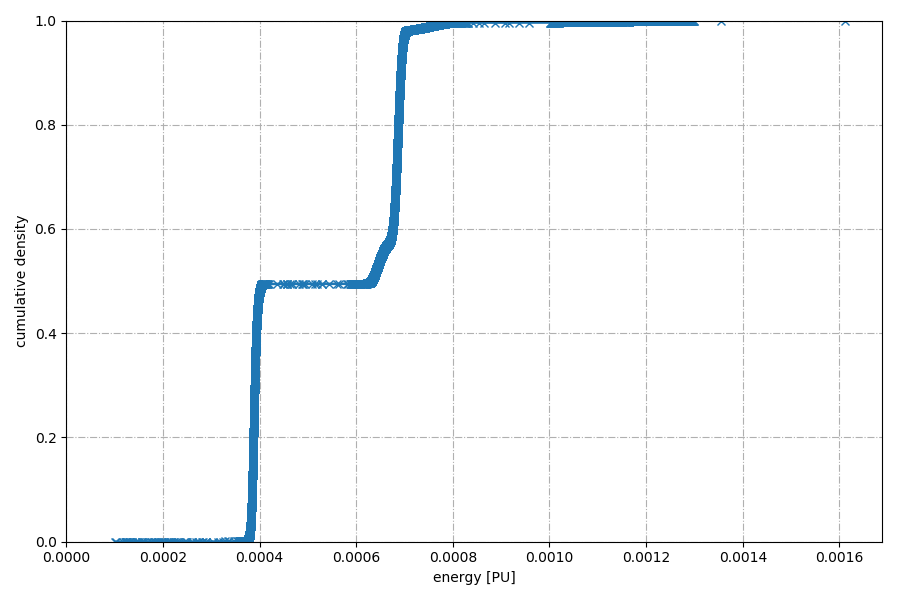
\includegraphics[width=0.6\textwidth]{pictures/results/same_combinations/csma_high_params/smoothed_channel_energy_cdf}}
		}
		\centerline{
			\subfloat[Channel Energy]{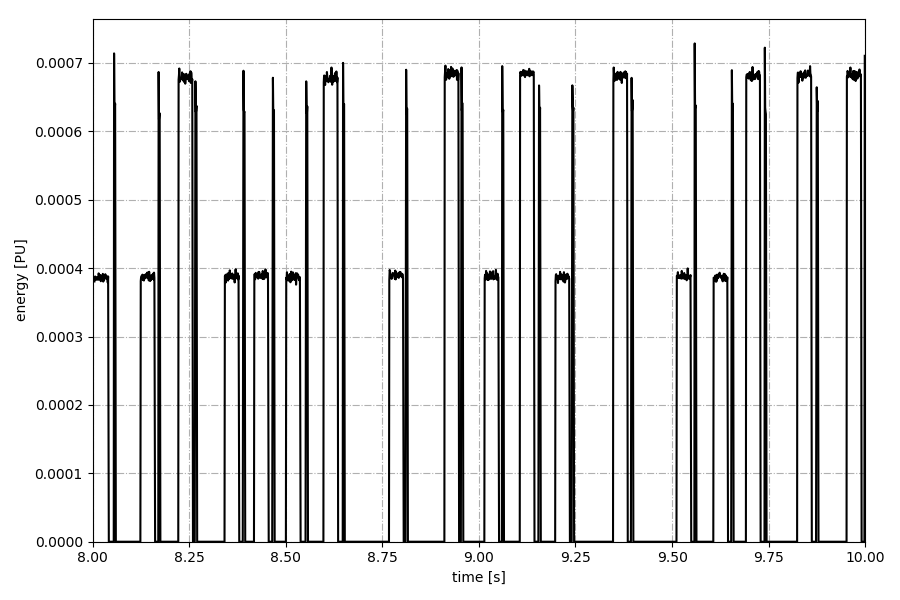
\includegraphics[width=0.6\textwidth]{pictures/results/same_combinations/csma_high_params/smoothed_channel_energy_level_4_line_chart}}
			\subfloat[Channel Energy CDF]{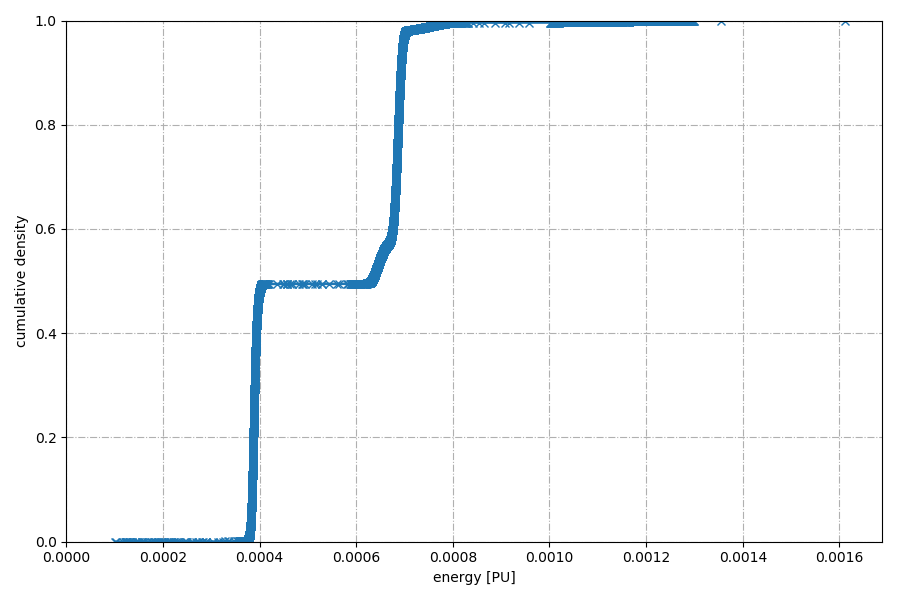
\includegraphics[width=0.6\textwidth]{pictures/results/same_combinations/csma_high_params/smoothed_channel_energy_cdf}}
		}
		\centerline{
			\subfloat[Logical Channel Occupation]{\includegraphics[width=0.6\textwidth]{pictures/results/same_combinations/csma_high_params/zoomed_channel_occupation_gantt_chart}}
			\subfloat[Total Backoff]{\includegraphics[width=0.6\textwidth]{pictures/results/same_combinations/csma_high_params/zoomed_channel_occupation_gantt_chart}}
		}		
	\end{center}
	\caption{Measurement results for the CSMA/CA with large parameter set}
\end{figure}